\documentclass[10pt,conference,compsoc]{IEEEtran}

\usepackage{amsmath}
\usepackage{balance}
\usepackage{booktabs}
\usepackage{graphicx}
\usepackage{microtype}
\usepackage{newtxtext,newtxmath}
\usepackage{url}
\usepackage{tikz}
\usepackage{pgfplots}
\pgfplotsset{compat=1.17}
\usetikzlibrary{arrows.meta,positioning}

\graphicspath{{../../figures/}}
% Website version. Build: tectonic talla_grasp_paper.tex

\title{Three Ways to Miss a Grasp: A Same-Metric Comparison of Rule-Based, Learned, and Zero-Shot Vision-Language Grasp Prediction}

\author{\IEEEauthorblockN{Anish Talla}
\IEEEauthorblockA{Lightridge High School and Academies of Loudoun\\
Virginia, United States\\
anish.talla99@gmail.com\\
\textit{Code and data:} \url{https://github.com/anishtalla27/Vision-Based-Grasping}}}

\begin{document}
\maketitle

\begin{abstract}
Rule-based, learned, and vision-language approaches to robotic grasp
prediction are usually evaluated under different inputs, output formats, and
scoring rules, which makes their published accuracies difficult to compare.
This paper provides a controlled evaluation of the three paradigms. A
detector-assisted heuristic, a fine-tuned convolutional network, and
zero-shot GPT-4o are tested on one object-wise split of the Cornell Grasping
Dataset, return the same grasp rectangle, and are scored by a single
implementation of the standard rectangle metric. Uncertainty is estimated by
resampling whole objects, because the test images are repeated views of only
35 objects. The learned predictor is the most accurate, the heuristic follows,
and the language model is far behind both. A shared failure taxonomy shows
that each system breaks at a different stage of the task. A follow-up
experiment then tests the most natural explanation for the language model's
result, that it identifies a suitable grasp but cannot write it as pixel
coordinates. When the same model only has to select one of several numbered
grasps drawn on the image, its accuracy remains at the level of random
selection. The limitation lies in choosing the grasp, not in expressing it.
\end{abstract}

\begin{IEEEkeywords}
robotic grasping, vision-language models, GPT-4o, Set-of-Mark prompting,
Cornell Grasping Dataset, clustered bootstrap
\end{IEEEkeywords}

\begin{figure*}[t]
\centering
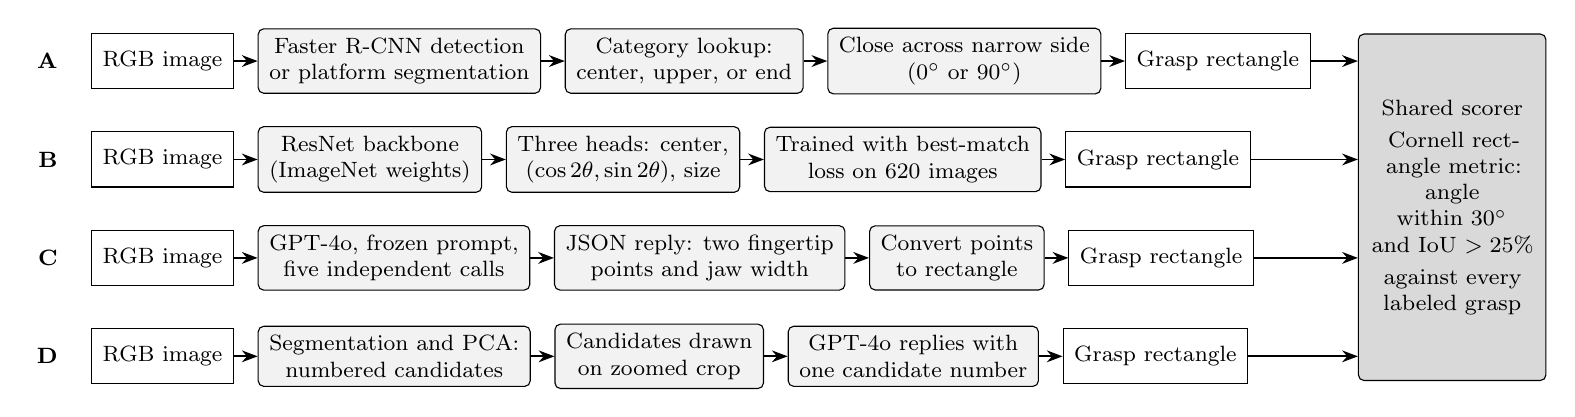
\begin{tikzpicture}[
  font=\footnotesize,
  box/.style={draw, rounded corners=2pt, minimum height=7mm, align=center,
              inner xsep=4pt, fill=gray!10},
  io/.style={draw, minimum height=7mm, align=center, inner xsep=4pt,
             fill=white},
  lab/.style={font=\footnotesize\bfseries, anchor=east},
  arr/.style={-{Stealth[length=2mm]}, semithick},
  node distance=5mm and 3mm]

% Row A
\node[lab] (la) at (0,0) {A};
\node[io, right=3mm of la] (a0) {RGB image};
\node[box, right=of a0] (a1) {Faster R-CNN detection\\or platform segmentation};
\node[box, right=of a1] (a2) {Category lookup:\\center, upper, or end};
\node[box, right=of a2] (a3) {Close across narrow side\\($0^\circ$ or $90^\circ$)};
\node[io, right=of a3] (a4) {Grasp rectangle};
\draw[arr] (a0)--(a1); \draw[arr] (a1)--(a2); \draw[arr] (a2)--(a3); \draw[arr] (a3)--(a4);

% Row B
\node[lab] (lb) at (0,-1.25) {B};
\node[io, right=3mm of lb] (b0) {RGB image};
\node[box, right=of b0] (b1) {ResNet backbone\\(ImageNet weights)};
\node[box, right=of b1] (b2) {Three heads: center,\\$(\cos 2\theta,\sin 2\theta)$, size};
\node[box, right=of b2] (b3) {Trained with best-match\\loss on 620 images};
\node[io, right=of b3] (b4) {Grasp rectangle};
\draw[arr] (b0)--(b1); \draw[arr] (b1)--(b2); \draw[arr] (b2)--(b3); \draw[arr] (b3)--(b4);

% Row C
\node[lab] (lc) at (0,-2.5) {C};
\node[io, right=3mm of lc] (c0) {RGB image};
\node[box, right=of c0] (c1) {GPT-4o, frozen prompt,\\five independent calls};
\node[box, right=of c1] (c2) {JSON reply: two fingertip\\points and jaw width};
\node[box, right=of c2] (c3) {Convert points\\to rectangle};
\node[io, right=of c3] (c4) {Grasp rectangle};
\draw[arr] (c0)--(c1); \draw[arr] (c1)--(c2); \draw[arr] (c2)--(c3); \draw[arr] (c3)--(c4);

% Row D
\node[lab] (ld) at (0,-3.75) {D};
\node[io, right=3mm of ld] (d0) {RGB image};
\node[box, right=of d0] (d1) {Segmentation and PCA:\\numbered candidates};
\node[box, right=of d1] (d2) {Candidates drawn\\on zoomed crop};
\node[box, right=of d2] (d3) {GPT-4o replies with\\one candidate number};
\node[io, right=of d3] (d4) {Grasp rectangle};
\draw[arr] (d0)--(d1); \draw[arr] (d1)--(d2); \draw[arr] (d2)--(d3); \draw[arr] (d3)--(d4);

% Shared scorer
\node[box, fill=gray!30, minimum height=44mm, right=6mm of a4.east, anchor=north west,
      yshift=3.5mm, text width=21mm] (sc)
      {Shared scorer\\[2pt] Cornell rectangle metric:\\angle within $30^\circ$\\and IoU $>25\%$\\[2pt] against every\\labeled grasp};
\draw[arr] (a4.east)--(a4.east -| sc.west);
\draw[arr] (b4.east)--(b4.east -| sc.west);
\draw[arr] (c4.east)--(c4.east -| sc.west);
\draw[arr] (d4.east)--(d4.east -| sc.west);
\end{tikzpicture}
\caption{The four systems. Each receives the same test image and produces a
grasp rectangle in the native $640\times480$ frame, and all rectangles pass
through one implementation of the Cornell metric. Systems C and D use the same
language model and differ only in what the model is asked to output.}
\label{fig:pipelines}
\end{figure*}

\section{Introduction}

Before a parallel-jaw gripper closes, a robot must settle three geometric
quantities: where the fingers land, how the gripper is rotated, and how far
the jaws open. That decision can be written by hand as a set of rules, learned
by a neural network from labeled examples, or requested from a
general-purpose vision-language model (VLM) that was never trained for
grasping. The three options differ greatly in setup cost. A rule needs no
labels, a network needs a labeled dataset and training, and a VLM needs only
a prompt. Their reported accuracies, however, are rarely comparable, because
the input, the output format, or the scoring rule changes from one method to
the next.

This paper treats the comparison as a measurement problem. One system of each
kind is built, and everything around the systems is held fixed. Each system
receives the same 123 held-out RGB images, returns the same rectangle
representation, and is scored against the same Cornell labels by one
implementation of the standard rectangle test \cite{jiang2011,lenz2015}.
Object identities, which the dataset does not provide, are reconstructed so
that no physical object appears in both training and test data. Because
several test images show the same object from different angles, all
statistics are computed over objects, not images. The VLM, whose output
varies between calls on identical input, is queried five times per image so
that this variation can be measured.

The contributions are as follows.
\begin{itemize}
\item A same-metric evaluation of a rule-based, a learned, and a zero-shot
VLM grasp predictor on a leak-free object-wise split, with object-clustered
confidence intervals and paired significance tests.
\item A shared failure taxonomy, together with a spatial check on the
predicted grasp center, that locates the stage at which each system fails.
\item A controlled follow-up experiment (System D) that removes the VLM's
coordinate output and tests whether its failure is one of expression or of
grasp selection.
\item A label-free geometric baseline that emerges from that experiment and
matches the detector-based heuristic.
\end{itemize}

The goal is not to exceed the state of the art. Dense grasp detectors already
report higher Cornell scores \cite{kumra2020}. The goal is to compare three
practical starting points under a test that does not change with the method.

\section{Related Work}

Jiang \emph{et al.} introduced the Cornell dataset and its rectangle
representation of a grasp, which stores the center, orientation, opening, and
jaw depth \cite{jiang2011}. Under the usual Cornell test, a prediction passes
when it lies within $30^\circ$ of a labeled grasp and its intersection over
union (IoU) with that grasp exceeds 25\% \cite{lenz2015}. Redmon and Angelova
regressed a single rectangle with a convolutional network and reported 84.9\%
object-wise accuracy using RGB-D input \cite{redmon2015}. GR-ConvNet and other
pixel-wise models report higher scores, although they produce a dense
prediction over the image and do not regress one rectangle \cite{kumra2020}.

VLM-based grasping systems generally avoid asking the language model for
final pixel coordinates. Set-of-Mark prompting has the model choose among
regions already marked on an image \cite{yang2024}. VLAD-Grasp has a VLM draw
the grasp and then recovers a pose through depth prediction, segmentation,
and point-cloud alignment \cite{kulshrestha2025}. System C in this paper tests
the simplest possible pipeline, in which GPT-4o is shown the image and asked
for the coordinates directly. System D then moves toward the Set-of-Mark
setting. The scores of both systems describe those two ways of querying the
model and do not bound what VLM-based grasping can achieve.

\section{Experimental Design}

Figure~\ref{fig:pipelines} summarizes the four systems. This section describes
the protocol and each system. All outcomes, including those from
development-stage checks, are reported in Section~\ref{sec:results}.


\subsection{Dataset, Split, and Metric}

The Cornell Grasping Dataset contains 885 RGB-D images of household objects,
most with several labeled positive grasp rectangles. Only the RGB channels
are used here. Two images were removed because their object boundaries could
not be resolved, which leaves 883.

The dataset does not include object identifiers, so they were reconstructed
from the frame sequence. The object was segmented from the photography
platform, and consecutive masks were compared using color and area
descriptors that tolerate rotation. The two possible errors are not equally
harmful. If two objects are merged, the combined group still stays within one
partition. If one object is divided in two, its images can leak into both
training and test data. The decision thresholds were therefore set to favor
merging. An automated first pass assigned a decision and a confidence level
to each ambiguous boundary, and a blind audit of 30 boundaries measured its
agreement with manual labels (Section~\ref{sec:res-split}). Every uncertain
decision and every high-risk ``different object'' decision was then resolved
manually, and a final check confirmed that no object appears in more than
one partition.

Each prediction is scored against every positive rectangle on its image, and
a match to any of them counts as correct. Before the evaluator was used at
scale, it was verified against hand-computed cases, rectangle round trips,
and an independent rasterized IoU calculation. All predictions are converted
to the native $640\times480$ coordinate frame before scoring.

\subsection{System A: Detector-Assisted Heuristic}

System A begins with a COCO-pretrained Faster R-CNN with a ResNet50-FPN-v2
backbone \cite{ren2015}. A fixed lookup table maps the detected category to a
center, upper, or end grasp, and the gripper closes across the narrow
dimension of the bounding box. The global opening and jaw-size constants were
calibrated on training labels only. Because the COCO vocabulary covers few
Cornell objects, a platform-segmentation fallback supplies a box when the
detector returns nothing. By construction, the system can output only
$0^\circ$ or $90^\circ$.

The system was revised once after its first test evaluation. Rendered
predictions showed that some accepted detections covered background clutter
instead of the object on the platform. A guard was added that requires the
detection to contain the centroid of the segmented object, and the global
constants were recalibrated on training data. Because test output prompted
this change, the corrected score is treated as post-hoc throughout, and the
pre-correction score is reported alongside it.

\subsection{System B: Learned Predictor}

System B replaces the ImageNet classifier of a ResNet \cite{he2016} with
separate heads for center, orientation, and size. The orientation head
predicts $(\cos 2\theta,\sin 2\theta)$, since a parallel-jaw grasp is
unchanged by a $180^\circ$ rotation. For images with several labels, the loss
is computed against every rectangle and only the best match is
backpropagated. Averaging over all valid labels could place the target
between two good grasps, at a location where no valid grasp exists.

Training proceeded in two rounds on the 620 training images, with affine
augmentation that moves the rectangle corners together with the pixels. In
the first round, a small custom CNN, ResNet18, and ResNet34 were each trained
once with a constant learning rate. The architecture, checkpoint, size-loss
weight, and the custom CNN's learning rate were selected on validation data,
and the selected model was frozen before the test split was opened.

The first round relied on a single seed and on the best of roughly one
hundred noisy validation epochs. The second round kept the model, loss, data,
and split, and changed only the training recipe: cosine learning-rate decay
over a fixed 100 epochs, an exponential moving average of the weights, three
seeds per architecture, and no checkpoint selection. Test-time augmentation
over eight dihedral views, combined by taking the medoid rectangle, was
adopted on the basis of validation accuracy alone. Four selection rules were
written down before the test split was opened a second time, and every
configuration that was evaluated on test data is reported.

\subsection{System C: Zero-Shot VLM}

System C sends the native RGB image to GPT-4o through OpenRouter
\cite{openai2024}, with no grasp-specific training. The prompt requests two
fingertip coordinates and a jaw width in JSON, which together define the
rectangle. The prompt was developed on 30 training images and frozen before
testing.

Each test image was submitted in five independent single-turn calls at the
provider's default temperature. Transport failures were retried. Replies that
arrived but failed to parse were not, because retrying them would convert a
single-call baseline into a best-of-several system. The primary score pools
the five exchangeable runs to estimate single-call accuracy. Best-of-five
accuracy is reported only as an upper bound, since it requires five calls and
an oracle that knows which call is correct.

\subsection{System D: Marked-Candidate Selection}

If GPT-4o can identify where to grasp but cannot express the location as
coordinates, removing the coordinate output should recover its choice. System
D shows the same model the same test images with candidate grasps drawn on a
zoomed crop (Fig.~\ref{fig:som}) and asks for the number of the candidate it
would use. Candidates are generated from the platform-segmentation mask
alone. Principal-component analysis gives the centroid, long axis, and
extent of the object, and candidates are placed at positions along the long
axis with four jaw-travel directions $45^\circ$ apart, so that every possible
grasp angle lies within the metric's tolerance of some candidate. Opening and
jaw width reuse System A's training-calibrated constants, and the numbering
is reshuffled on every call. Because the menu is fixed before the model sees
it, each run has a known floor (the expected accuracy of a uniformly random
choice) and a known ceiling (the share of images on which any candidate
passes).

Three menus were evaluated, each on the full test split with five repeats.
The first has twelve marks at three positions. The second has four marks at
the centroid only, drawn at real size. The third has the same four marks
drawn at one uniform length, with a prompt stating that length is not to
scale. The last two menus control for a confound: on thin objects the
correct marks are the smallest ones on the image, so a preference for large
marks would be indistinguishable from a preference for a particular grasp
direction. The prompt was developed on 30 training images for parse rate and
glyph legibility only, and each menu was run on the test split exactly once.

\begin{figure}[t]
\centering
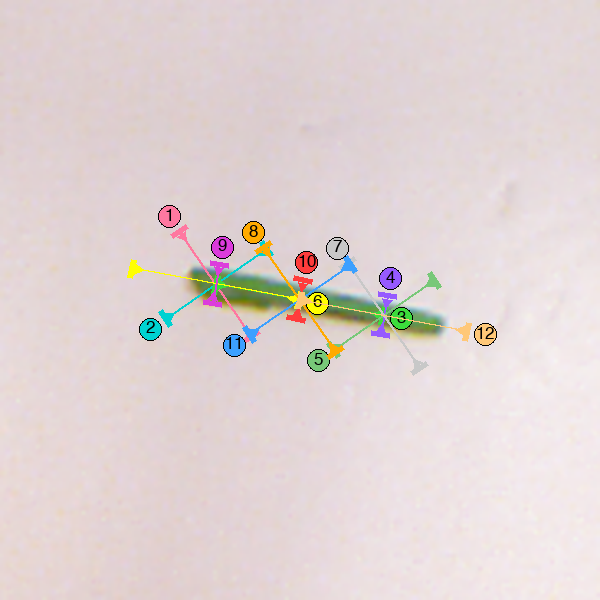
\includegraphics[width=0.78\columnwidth]{som_0129.png}
\caption{A System D input from the twelve-mark menu. Each numbered mark is a
candidate grasp, with pads at the two fingertip positions. On all five
repeats the model chose mark 6, the pinch along the length of the object.
Mark 10, which crosses the object at its center, passes the metric.}
\label{fig:som}
\end{figure}

\subsection{Statistical and Failure Analysis}

The 123 test images are repeated views of 35 unseen objects and are not
independent samples. All 95\% confidence intervals therefore come from 20,000
object-clustered bootstrap resamples, in which every view of an object and
all five VLM calls on each view are resampled together. Paired differences
between systems use the same resamples, and significance is assessed with
20,000 object-level label-swap permutations.

For the failure analysis, each attempt receives exactly one label: correct,
angle criterion failed, overlap criterion failed, both failed, or no
prediction. A second check records whether the predicted center falls inside
the convex hull of all labeled grasp corners on the image. This is a loose
spatial test of whether a prediction is near any annotated grasp, and it
makes no claim about physical grasp success.

\section{Results}
\label{sec:results}

\subsection{Data Split and Boundary Audit}
\label{sec:res-split}

Table~\ref{tab:split} gives the final split, generated with seed 42. In the
blind 30-boundary audit, the automated first pass agreed with manual labels
on 86.7\% of the boundaries it marked confident and on 40.0\% of those it
marked uncertain. The low agreement on uncertain cases is the reason all of
them were decided manually.

\begin{table}[t]
\caption{Object-wise Cornell split.}
\label{tab:split}
\centering
\begin{tabular}{lrr}
\toprule
Partition & Objects & Images \\
\midrule
Train & 164 & 620 \\
Validation & 35 & 140 \\
Test & 35 & 123 \\
\midrule
Total & 234 & 883 \\
\bottomrule
\end{tabular}
\end{table}

\subsection{Overall Accuracy}

Table~\ref{tab:accuracy} and Fig.~\ref{fig:accuracy} report test accuracy for
every system, and Table~\ref{tab:paired} reports the paired differences. The
ordering is unambiguous. The learned predictor leads, the heuristic follows,
and single-call GPT-4o is far behind both, including the heuristic's
pre-correction score. Every paired difference between the three paradigms
excludes zero, and this holds even when GPT-4o is credited with its
best-of-five upper bound. Weighting each object equally instead of each image
(last column of Table~\ref{tab:accuracy}) changes the size of the gaps but
not their order. Clustering by object widens every interval relative to an
image-level analysis, which shows how much an image-level analysis would
overstate the precision of a 123-image test set.

\begin{table}[t]
\caption{Test accuracy with object-clustered 95\% confidence intervals.
``Obj.-wt.'' gives each of the 35 test objects equal weight.}
\label{tab:accuracy}
\centering
\footnotesize
\begin{tabular}{lrrr}
\toprule
System & Acc. & 95\% CI & Obj.-wt. \\
\midrule
A: heuristic, pre-correction & 40.7 & -- & -- \\
A: heuristic, post-hoc fix & 57.7 & [46.2, 68.2] & 51.3 \\
B: ResNet18, round 1 & 79.7 & [70.8, 87.1] & 75.4 \\
B: ResNet34, round 2, 3 seeds & \textbf{84.0} & [73.9, 92.1] & -- \\
C: GPT-4o, single call & 12.4 & [8.0, 17.4] & 10.5 \\
C: GPT-4o, best of five & 35.0 & [24.6, 45.5] & -- \\
\bottomrule
\end{tabular}
\end{table}

\begin{figure}[t]
\centering
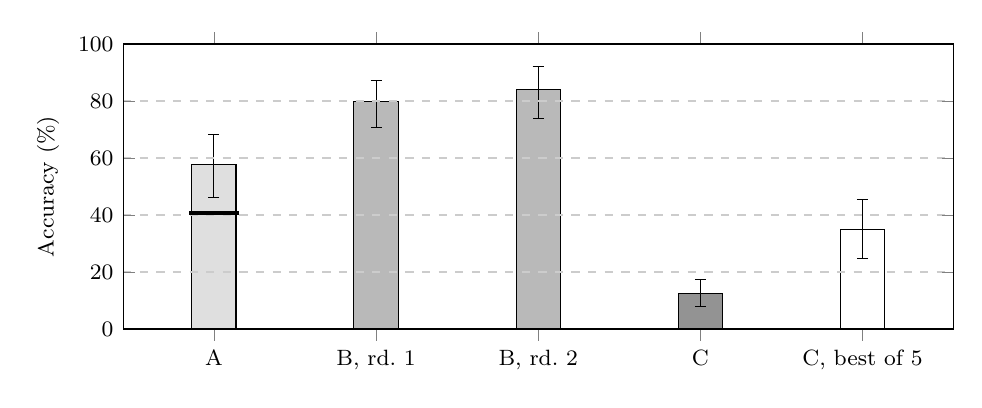
\begin{tikzpicture}
\begin{axis}[
  width=\columnwidth, height=5.2cm,
  ybar, bar width=16pt,
  ymin=0, ymax=100,
  ylabel={Accuracy (\%)},
  symbolic x coords={A,B1,B2,C,Cb},
  xtick={A,B1,B2,C,Cb},
  xticklabels={{A},{B, rd.\ 1},{B, rd.\ 2},{C},{C, best of 5}},
  tick label style={font=\footnotesize},
  label style={font=\footnotesize},
  enlarge x limits=0.14,
  ymajorgrids=true, grid style={dashed,gray!40},
  axis on top,
]
\addplot[fill=gray!25,draw=black,bar shift=0pt,error bars/.cd,y dir=both,y explicit]
  coordinates {(A,57.7) += (0,10.5) -= (0,11.5)};
\addplot[fill=gray!55,draw=black,bar shift=0pt,error bars/.cd,y dir=both,y explicit]
  coordinates {(B1,79.7) += (0,7.4) -= (0,8.9)};
\addplot[fill=gray!55,draw=black,bar shift=0pt,error bars/.cd,y dir=both,y explicit]
  coordinates {(B2,84.0) += (0,8.1) -= (0,10.1)};
\addplot[fill=gray!85,draw=black,bar shift=0pt,error bars/.cd,y dir=both,y explicit]
  coordinates {(C,12.4) += (0,5.0) -= (0,4.4)};
\addplot[fill=white,draw=black,bar shift=0pt,error bars/.cd,y dir=both,y explicit]
  coordinates {(Cb,35.0) += (0,10.5) -= (0,10.4)};
\addplot[only marks,mark=-,mark size=9pt,very thick,draw=black]
  coordinates {(A,40.7)};
\end{axis}
\end{tikzpicture}
\caption{Test accuracy with object-clustered 95\% intervals. The horizontal
rule on bar A marks the heuristic's pre-correction score. The white bar is an
upper bound that requires five calls and an oracle.}
\label{fig:accuracy}
\end{figure}

\begin{table}[t]
\caption{Paired accuracy differences in percentage points, with
object-clustered bootstrap intervals and permutation $p$-values.}
\label{tab:paired}
\centering
\footnotesize
\begin{tabular}{lrrr}
\toprule
Comparison & Diff. & 95\% CI & $p$ \\
\midrule
B round 1 $-$ A & 22.0 & [9.7, 35.1] & 0.0031 \\
B round 2 $-$ A & 26.3 & [14.8, 38.3] & 0.0002 \\
B round 2 $-$ B round 1 & 4.3 & [$-5.8$, 13.7] & n.s. \\
A $-$ C, single call & 45.4 & [33.8, 55.6] & $<$0.0001 \\
A $-$ C, best of five & 22.8 & [9.2, 35.6] & 0.0060 \\
\bottomrule
\end{tabular}
\end{table}

\subsection{Stability of the Learned Predictor}

Table~\ref{tab:round2} places the two training rounds side by side. The
second round does not show a statistically reliable improvement over the
first (Table~\ref{tab:paired}). Its value is that it measures the uncertainty
the first round left unmeasured. Rerunning the first-round recipe at new
seeds produced higher scores than the original run, which indicates that
79.7\% was a low draw from that recipe. The first round also suggested that
ResNet18 outperformed ResNet34 by nine points, but under the stable recipe
the two architectures are level on validation data (81.2\% and 81.4\%) and
within 1.4 points on test data. That apparent architecture effect was
run-to-run variation, and a single-seed comparison would have reported it as
a finding.

\begin{table}[t]
\caption{System B on the 123 test images. Round 1 reports the
validation-selected checkpoint. Round 2 reports final averaged weights with
test-time augmentation, as a mean over three seeds.}
\label{tab:round2}
\centering
\footnotesize
\begin{tabular}{llr}
\toprule
Round & Configuration & Test acc. (\%) \\
\midrule
1 & ResNet18, seed 42 & 79.7 \\
1 & ResNet34, seed 42 & 70.7 \\
1 & Custom CNN, seed 42 & 23.6 \\
1 recipe & ResNet18, seeds 0 and 1 & 82.9, 80.5 \\
2 & ResNet18 (83.7, 80.5, 83.7) & 82.6 \\
2 & ResNet34 (84.6, 83.7, 83.7) & \textbf{84.0} \\
\bottomrule
\end{tabular}
\end{table}

\subsection{Failure Patterns}

Table~\ref{tab:taxonomy} separates the systems more clearly than accuracy
does, because each system loses most of its attempts in a different row.
System A's angle-only failures are consistent with a rule restricted to two
orientations: the rectangle overlaps a labeled grasp, but the object lies
diagonally. System B rarely misses on angle alone, and most of its failures
are overlap-only, so placement and sizing are its remaining weakness. System
C fails both criteria on the majority of its calls, which indicates that its
rectangles are usually not near a labeled grasp at all.

\begin{table}[t]
\caption{Shared failure taxonomy. Entries are counts, with percentages of
all attempts in parentheses. Round 1 model for System B.}
\label{tab:taxonomy}
\centering
\footnotesize
\begin{tabular}{lrrr}
\toprule
Outcome & A ($n=123$) & B ($n=123$) & C ($n=615$) \\
\midrule
Correct & 71 (57.7) & 98 (79.7) & 76 (12.4) \\
Angle failed only & 13 (10.6) & 4 (3.3) & 85 (13.8) \\
Overlap failed only & 18 (14.6) & 15 (12.2) & 88 (14.3) \\
Both failed & 13 (10.6) & 6 (4.9) & 365 (59.3) \\
No prediction & 8 (6.5) & 0 (0.0) & 1 (0.2) \\
\bottomrule
\end{tabular}
\end{table}

The center-hull check in Table~\ref{tab:hull} supports that reading. Systems
A and B place almost all of their centers within the region spanned by the
labeled grasps, while System C places more than half of its centers outside
it. The three rates are not a measure of the same skill. System A starts from
a detected or segmented object, and System B was trained on Cornell images,
whereas System C may place its coordinates anywhere in the frame. The check
is used only to locate the stage at which System C's failures begin.
Figure~\ref{fig:comparison} shows the behavior on one test image.

\begin{table}[t]
\caption{Predicted centers outside the convex hull of all labeled grasp
corners, and agreement among System C's five calls per image.}
\label{tab:hull}
\centering
\footnotesize
\begin{tabular}{lr}
\toprule
Quantity & Value \\
\midrule
A: centers outside hull & 8 of 115 (7.0\%) \\
B: centers outside hull & 8 of 123 (6.5\%) \\
C: centers outside hull & 328 of 614 (53.4\%) \\
\midrule
C: range of the five runs & 9.8\% to 14.6\% \\
C: mean pairwise rectangle agreement & 22.0\% \\
C: mean pairwise IoU & 0.13 \\
C: images where all five calls fail & 80 of 123 \\
C: images where all five calls pass & 1 of 123 \\
C: images with mixed outcomes & 42 of 123 \\
\bottomrule
\end{tabular}
\end{table}

\begin{figure}[t]
\centering
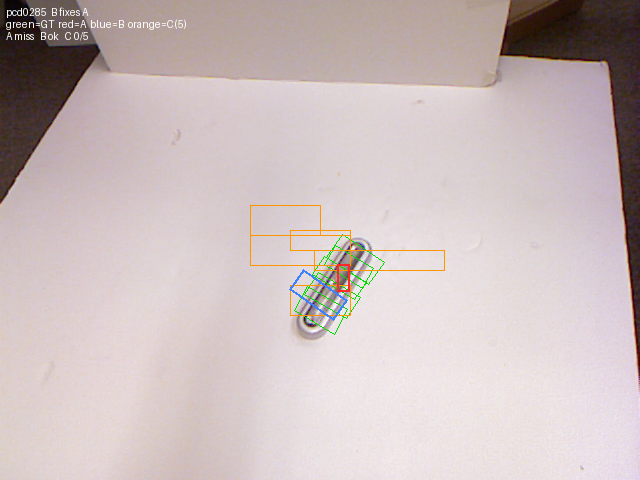
\includegraphics[width=\columnwidth]{compare_0285.png}
\caption{One test image in the shared coordinate frame. Labeled grasps are
green, System A is red, System B is blue, and System C's five calls are
orange.}
\label{fig:comparison}
\end{figure}

System C is also inconsistent with itself (lower half of
Table~\ref{tab:hull}). On roughly a third of the test images, identical
pixels produced a passing grasp on some calls and a failing grasp on others.
A single-call score therefore understates the spread a user would observe,
and the best-of-five figure cannot be realized without an external signal
that identifies the correct call.

\subsection{System D: Selection Among Marked Candidates}

Table~\ref{tab:menus} reports the three menus. On none of them does the
model's accuracy differ from random selection among the same candidates,
although a passing candidate was available on most images. Removing the
coordinate output therefore did not recover a correct choice. All 560
submitted replies parsed, so the result does not reflect a formatting
problem.

\begin{table}[t]
\caption{System D on three candidate menus, five repeats each. ``Diff.'' is
accuracy minus the random floor with its object-clustered 95\% interval.
``Long axis'' is the share of calls choosing a grasp whose jaws travel along
the object's long axis (chance is 25\%).}
\label{tab:menus}
\centering
\footnotesize
\setlength{\tabcolsep}{2.6pt}
\begin{tabular}{lrrrrr}
\toprule
Menu & Acc. & Floor & Ceil. & Diff. [95\% CI] & Long axis \\
\midrule
12 marks & 18.7 & 20.1 & 79.7 & $-1.4$ [$-6.6$, 4.0] & 70\% \\
4 marks, real size & 26.5 & 24.6 & 65.9 & $+1.9$ [$-2.2$, 6.3] & 41\% \\
4 marks, uniform & 22.3 & 24.6 & 65.9 & $-2.3$ [$-6.3$, 1.7] & 45\% \\
\midrule
\multicolumn{6}{l}{Geometric rule alone (centroid, short axis): 55.3 [41.8, 68.0]} \\
\bottomrule
\end{tabular}
\end{table}

The model's choices are nevertheless systematic. On every menu it selected
the long-axis direction well above the chance rate, and the preference
persisted when all marks were drawn at the same length, which rules out mark
size as the explanation. On the twelve-mark menu, a single candidate type,
the pinch along the long axis near one end of the object, received 61\% of
all choices although it passes on only 17\% of images. The short-axis
candidate at the centroid, which passes on 55\% of images, was chosen in 17\%
of calls on the uniform menu. The model's written justifications described
the chosen grasp in plausible terms, such as gripping ``the narrow top edge
near the center of mass'', and its stated confidence was ``high'' on 556 of
560 calls, of which 21\% were correct.

The experiment also produced an unplanned baseline. Always selecting the
centroid candidate that closes across the short axis, with no model involved,
scores 55.3\% (Table~\ref{tab:menus}). This is level with System A and
requires neither a detector nor a category table.

\section{Discussion}

\subsection{Interpretation}

The cost of each approach and its accuracy were ordered in the same way on
this benchmark. The learned predictor required labels and training and was
the most accurate. The heuristic required no labels and reached a moderate
score, limited mainly by its two fixed orientations. Zero-shot GPT-4o
required only a prompt and did not produce usable rectangles. That last
result applies to direct coordinate prompting on this setup and should not be
generalized to VLM grasping as a whole. Set-of-Mark and VLAD-Grasp both avoid
asking the model for final coordinates, and both add components that System C
lacks \cite{yang2024,kulshrestha2025}.

The System C results initially suggested a coordinate-binding hypothesis. In
a sample of its failures, the written rationale named a plausible part of the
object while the coordinates landed elsewhere, and more than half of its
centers fell outside the labeled region. Under that hypothesis, the model
recognizes a suitable region in language and loses it when mapping the answer
to pixels. System D tested the hypothesis directly, and the hypothesis was
not supported. With coordinates removed and a passing candidate available on
most images, the model still chose at the level of chance, and it kept its
preference for closing along the long axis on menus with no end-straddling
candidates and with uniform mark sizes.

A geometric reading of that preference is available. In a top-down
photograph, two fingertip pads placed across the end of an elongated object
appear to pinch a narrow part. In three dimensions, one of those fingers
would land on top of the object. The failure is therefore better described
as grasp reasoning from a single two-dimensional view than as a failure to
bind text to coordinates.

\subsection{Limitations}

The study uses one object-wise split of a small benchmark, RGB input without
depth, and no robot trials. Cornell annotations are not exhaustive, so a
rectangle that fails the metric could still succeed on a physical object.
Development effort was uneven: System B received three architectures,
validation-based tuning, and a second training round, whereas Systems C and D
each used one frozen prompt. The test split was opened twice for System B,
once per round, under rules fixed in advance. System D used one glyph style
and one candidate generator. An early formatting check on about 550 grasp
rectangles probably included a few images that later entered the test
partition, although no parameter or rule was derived from that check.
Finally, System A's correction was prompted by test output, so comparisons
that use its 57.7\% score are post-hoc and 40.7\% remains its clean result.
Confirming these findings would require a fresh split or a second dataset.

\section{Conclusion}

Published accuracies for rule-based, learned, and language-model grasp
predictors are difficult to compare because each is usually measured under
its own conditions. This paper removed that obstacle for one benchmark. Three
systems, one from each paradigm, were given the same images, the same output
representation, the same scorer, and a split in which no object is shared
between training and test data, and all uncertainty was computed over
objects instead of images.

Under those conditions the ranking is clear and statistically robust. A
fine-tuned ResNet is correct on roughly four of five images of unseen objects,
a hand-written heuristic on somewhat more than half, and zero-shot GPT-4o on
about one in eight. The more useful result is where each system fails. The
heuristic finds the object but cannot represent its angle. The network finds
the angle and misses on placement. The language model usually fails before
either distinction matters, because its rectangle is not near any labeled
grasp, and it gives different answers to identical input.

The follow-up experiment changes how that last failure should be understood.
Offered a menu of drawn grasps, most of which contained a correct option,
GPT-4o chose no better than chance on three different menus and consistently
preferred a pinch along the object's long axis, with high stated confidence.
The model's difficulty is selecting a grasp from a single top-down view, not
writing the grasp as numbers. For practitioners, this suggests that wrapping
a general-purpose VLM in a better output format will not by itself yield a
grasp planner, and that a simple geometric rule on a segmentation mask is a
useful baseline: it matches the detector-based heuristic at lower cost and
far exceeds the language model.

Two methodological points apply beyond grasping. Clustering the statistics by
object widened every interval, and repeating training across seeds removed an
architecture effect that a single run had suggested. Both checks cost little
and changed what could be claimed. The main open question is whether depth
input, or a model with a stronger three-dimensional prior, changes the
language model's choice. All code, the split, the raw model replies, and the
scoring scripts are available in the project repository.

\section*{Acknowledgment}

OpenAI Codex helped restructure, shorten, and edit an earlier conference
version of this manuscript from the author's existing report, code, and
verified results. Anthropic Claude Code helped with code development, made
the first-pass calls on ambiguous object boundaries, implemented the second
training round and System D under the author's design, and helped edit this
version. The author designed the study, made the research decisions, ran and
checked the experiments, verified the citations and numerical claims, and
approved the final text. GPT-4o was evaluated separately as Systems C and D.

\balance
\begin{thebibliography}{00}

\bibitem{jiang2011}
Y. Jiang, S. Moseson, and A. Saxena, ``Efficient grasping from RGBD images:
Learning using a new rectangle representation,'' in \emph{Proc. IEEE Int.
Conf. Robot. Autom. (ICRA)}, 2011, pp. 3304--3311.

\bibitem{lenz2015}
I. Lenz, H. Lee, and A. Saxena, ``Deep learning for detecting robotic
grasps,'' \emph{Int. J. Robot. Res.}, vol. 34, nos. 4--5, pp. 705--724, 2015.

\bibitem{redmon2015}
J. Redmon and A. Angelova, ``Real-time grasp detection using convolutional
neural networks,'' in \emph{Proc. IEEE Int. Conf. Robot. Autom. (ICRA)},
2015, pp. 1316--1322.

\bibitem{kumra2020}
S. Kumra, S. Joshi, and F. Sahin, ``Antipodal robotic grasping using
generative residual convolutional neural network,'' in \emph{Proc. IEEE/RSJ
Int. Conf. Intell. Robots Syst. (IROS)}, 2020, pp. 9626--9633.

\bibitem{yang2024}
J. Yang \emph{et al.}, ``Set-of-Mark prompting unleashes extraordinary
visual grounding in GPT-4V,'' \emph{arXiv:2310.11441}, 2023.

\bibitem{kulshrestha2025}
M. Kulshrestha \emph{et al.}, ``VLAD-Grasp: Zero-shot grasp detection via
vision-language models,'' \emph{arXiv:2511.05791}, 2025.

\bibitem{ren2015}
S. Ren, K. He, R. Girshick, and J. Sun, ``Faster R-CNN: Towards real-time
object detection with region proposal networks,'' in \emph{Adv. Neural Inf.
Process. Syst.}, vol. 28, 2015.

\bibitem{he2016}
K. He, X. Zhang, S. Ren, and J. Sun, ``Deep residual learning for image
recognition,'' in \emph{Proc. IEEE Conf. Comput. Vis. Pattern Recognit.
(CVPR)}, 2016, pp. 770--778.

\bibitem{openai2024}
OpenAI, ``GPT-4o system card,'' \emph{arXiv:2410.21276}, 2024.

\end{thebibliography}

\end{document}
